\section{Planned Validation}
\label{sec:plan}

이 절의 결과 칸은 모두 비워 둔 예정 칸(\todoexp)이며, 판정 기준은 실행 전에 고정한다. 각 표의 캡션에 기대하는 결과와 그 결과가 지지하거나 반박하는 주장을 적는다. 기대와 다른 결과가 나와도 같은 표에 그대로 보고한다. 과금되는 실험은 사용자의 명시적 허락 뒤에만 돈다. 순서는 ``먼저 빼고, 필요하면 넣는다''를 따른다. 상위 계획기 단독을 먼저 다듬고 한계를 잰 뒤, 한계가 트리거 기준을 넘을 때만 VLA 층을 넣는다.

\subsection{검증 사다리}
\label{sec:ladder}
단계와 넘는 기준은 \cref{tab:ladder}에 있다. 1단계(이번 마일스톤: 결정 수집 $\rightarrow$ 강화 $\rightarrow$ 최종 35B $\rightarrow$ 평가)를 먼저 넘고, 2단계의 V0--V4는 \cref{sec:plan_limits}의 트리거가 걸릴 때만 연다.
\begin{table*}[t]
\centering
\scriptsize
\setlength{\tabcolsep}{3pt}
\begin{tabular}{@{}p{0.12\linewidth}p{0.38\linewidth}p{0.30\linewidth}p{0.14\linewidth}@{}}
\toprule
단계 & 무엇을 하나 & 넘는 기준(초안) & 상태 \\
\midrule
\multicolumn{4}{@{}l}{\textbf{1단계: 상위 계획기 단독(실행기와 함께) --- 이번 마일스톤}} \\
U0 & 8B 경향: 시뮬 참값 LoRA, 동기 단독 형식 & 오프라인 접근 오차 $\le$ 영샷의 절반, 폐루프 성공 $\ge1$ & 끝(\tentative{4/4}) \\
(1) 결정 & 출력 형식 두 줄기(E-PT/ND: 깊이 사용 D 대 RGB만 R) & DEV, OOD-H(좁게·넓게) 접근 오차 & \tentative{진행 중} \\
(1) 결정 & 손으로 준 정보(E-STRIP8 $\rightarrow$ L8-X에서 E-STRIP8b) & DEV·OOD 비열등, 공정 짝 비교 & 잠정 NOT\_NEEDED \\
(1) 결정 & 데이터 구성(E-DIST8 6팔: L8 / L8-D / L8-D + 공개 3D $\times$ 공개 픽셀 유무) & 수준마다 픽셀 짝 효과, DEV·OOD-H/O/D & \tentative{등록 전} \\
(1) 결정 & 공개 데이터 경로(작전 T: 좌표계 만들기 대 카메라 없는 조종; E-OPEN8) & L8-X에서 같은 조건 짝 비교, 누수 0 & \tentative{결정 대기} \\
(1) 결정 & 35B 학습 길이(E-TEACH-35B, 에폭마다 오프라인 평가) & 에폭 곡선 & \tentative{진행 중} \\
(1.5) 강화 & 선정된 방법마다 기본 성능 올리기(문헌 + 8B 사전 등록 짝 시험) & 효과가 확인된 것만 최종 레시피에 & \tentative{예정} \\
(2) 최종 & 35B-A3B 소규모 학습, 줄기 D와 R 두 판 & H-L 기준(\cref{sec:hl}) & \tentative{예정} \\
(3) 평가 & DEV, OOD-H/O/D/T(/S), 한계 지도(\cref{sec:plan_limits}) & 기술 지표, 트리거 판단의 근거 & \tentative{예정} \\
병행 & 자동 맥락: 사람이 쓴 맥락을 자동 값으로 하나씩 교체 & 참값 대비 오차, 폐루프 비열등 & \tentative{예정} \\
\midrule
\multicolumn{4}{@{}l}{\textbf{2단계: 한계가 트리거를 넘을 때만 --- VLA 층(두 모델 원래 형식 + 늘 섞기)}} \\
V0 & VLA 재학습(그리퍼 질문, 실데이터 먼 구간 분기 75\%) & 재학습 관문(결정 정확도 비열등, 재적재 일치) & 보류 \\
V1 & VLA 단독 폐루프, DEV 12편(런타임 멈춤 고리 수정 뒤) & 성공 $\ge$ \tentative{4/12} & 보류 \\
V2 & 목표$\rightarrow$결정 변환과 혼합 가중 규칙(무료 시뮬) & 방향 양자화 오차, 낡은 목표에서 VLA 가중 증가, 충돌 0 & 보류 \\
V3 & 결합 폐루프: 상위 + VLA 대 상위 단독 대 VLA 단독, DEV 40 짝 & \cref{tab:couple}의 판정 & 보류 \\
V4 & 유료 결합(Astra 상위) & 사용자 허락 뒤 & 보류 \\
\bottomrule
\end{tabular}
\caption{\textbf{검증 사다리.} 1단계(결정 수집, 강화, 최종 35B, 평가)를 먼저 넘고, 2단계(V0--V4)는 \cref{sec:plan_limits}의 트리거가 걸릴 때만 연다. 2단계의 코드와 계획은 보존한다. 실데이터 먼 구간 분기(E-SR1e)는 진행 중인 팔만 마무리한다. 유료는 사용자 허락 뒤에만 돈다.}
\label{tab:ladder}
\end{table*}

\subsection{이번 마일스톤: 결정 모으기 $\rightarrow$ 강화 $\rightarrow$ 최종 35B}
\label{sec:milestone}
이번 마일스톤의 목표는 각 실험의 최선을 모아 최종 35B-A3B를 그 방법론과 데이터로 소규모 학습하고 평가하는 것이다(정본 §98 보충 1). 순서는 다섯이다. (1) \emph{결정 수집}: 입력 형식(손으로 준 정보, L8-X에서 재검증), 출력 형식(E-PT/ND), 데이터 구성(E-DIST8, E-OPEN8, 작전 T), 학습 길이(35B 에폭 곡선)를 정한다. (1.5) \emph{강화}: 선정된 방법마다 기본 성능을 올릴 방법(데이터 혼합 비율·커리큘럼, 증강, LoRA 대상·랭크, 학습률·에폭, 라벨 품질 거르기, 자기 점검 출력, 추론 설정)을 문헌에서 찾고, 싼 8B 사전 등록 짝 시험으로 확인된 것만 최종 레시피에 넣는다. (2) \emph{최종 35B 소규모 학습}: 줄기 D와 R 두 판을 같은 조건으로 학습한다. (3) \emph{평가}: DEV, OOD-H(좁게·넓게)/O/D/T, 한계 지도, H-L 기준. (4) \emph{다음 결정}: 한계가 트리거를 넘으면 2단계 VLA 결합으로, 아니면 대규모 학습과 실물 준비로 간다.

\textbf{E-DIST8}은 데이터 구성을 정하는 요인 실험이다(8B, 무료, 팔마다 같은 걸음·표본 수). 데이터 기반 3수준(L8, L8-D, L8-D + 공개 3D 질의응답·좌표계 명시 조종)과 공개 픽셀 흐름 유무 2수준을 곱한 6팔이다. 픽셀이 도움인지 방해인지를 세 수준 각각에서 짝으로 판정한다. 평가는 DEV, OOD-H(좁게·넓게), OOD-O/D이며, 줄기 D·R의 짝 비교도 같은 조건으로 붙인다(\tentative{등록 전}).

두 가지 절차 규칙을 둔다. 안을 버리기 전에는 한 번 재검증한다. 재검증으로 살아난 안은 기존 안을 바로 대체하지 않는다. 같은 데이터·학습량·평가 세트·시드·판정 규칙으로 사전 등록한 짝 비교를 한 번 더 거친 뒤에만 고른다. 손으로 준 정보의 유지·제거, 좌표계 만들기 대 카메라 없는 조종이 여기에 해당한다.

\subsection{가설 H-L: 특화 학습한 상위 모델}
\label{sec:hl}
\tentative{Astra는 한 호출에 수 초라 실시간 참여와 감독에 너무 느리다. 일반 능력은 낮아도 말단과 로봇·장면의 관계와 이동의 상관에 특화해 학습한 상위 모델은 더 빠르고, 우리 과제에서는 비슷하거나 더 나을 것이다.} 판정 기준 초안은 셋이다. \emph{빠르다}: 지연 p50 $\le$ \tentative{2\,s}이자 Astra의 1/3 이하. \emph{비슷하다}: DEV 짝 시드에서 Astra 단독과의 성공 차가 \tentative{3/40} 안. \emph{더 좋다}: 접근 목표 오차가 Astra(중앙 약 \tentative{14\,mm}) 이하이고, 7--10\,cm 목표 어긋남 알아채기가 Astra의 \tentative{0/13}보다 높다. 8B 경향 시험은 분포 안에서 첫 근거를 주었지만 지연 기준에는 못 미쳤다. 35B-A3B는 준비 측정에서 동기 단독 요청 p50 \tentative{1.11\,s}로 응답해, 영샷 기준으로는 지연 기준 안에 있다. 다만 학습 뒤 답 길이에 따라 달라지고, 과제 성능은 아직 모른다(\cref{sec:evidence}). 위험은 드문 상태의 복구 추론을 잃는 것이다. 그래서 학생이 간 틀어진 상태의 복구 라벨을 반드시 넣고, 일반성은 학습에 쓰지 않은 OOD 세트로 잰다.

\subsection{1단계의 한계 지도와 2단계 트리거}
\label{sec:plan_limits}
상위 단독 폐루프의 모든 판에서 네 가지를 기술 지표로 기록한다. (i) \emph{분포 밖}: OOD-H(본 적 없는 탁자 높이), OOD-O(보류한 물체 범주), OOD-D(보류 풀의 방해물·재질·조명)의 성공과 접근 오차. (ii) \emph{실행 중 교란}: 편 도중 대상이 3--8\,cm 순간 이동했을 때 다음 몇 호출 안에 목표를 고치는지, 나르는 중 그리퍼가 열려 물체를 놓쳤을 때 알아채고 다시 잡는지. (iii) \emph{접촉 정밀도}: 첫 닫기 때 손끝과 대상 중심의 xy 차, 닫기 높이 오차, 빈손 닫힘 수, 놓은 위치의 오차와 똑바름. (iv) \emph{시간}: 편당 벽시계(상위 지연 합 + 실행기 움직임 + 대기)와 호출 수. 움직임 시간과 대기 시간을 나눠 적는다. 교란 주입은 동기 단독 러너에 아직 없어 구현과 시험 뒤에 등록한다.

2단계는 한계가 아래 트리거 가운데 하나를 넘을 때만 연다. 문턱은 초안이며 1단계 결과 전에 사전 등록으로 고정한다. \textbf{T-lat}: 실패한 편 가운데 원인이 기다림(상위가 답하는 동안 상황이 바뀜)으로 분류된 비율이 \tentative{초안 문턱} 이상. \textbf{T-wall}: 편당 벽시계가 같은 장면의 스크립트 규칙 기준선 대비 \tentative{초안 배수} 이상이고, 그 대부분이 대기 시간. \textbf{T-contact}: 교란이나 접촉 정밀도의 실패가 상위의 답 간격보다 짧은 시간 척도에서 일어남(예: 미끄러짐을 다음 호출 전에 되잡아야 하는 경우). 트리거가 걸리지 않으면 VLA 층은 넣지 않고, 그 결과를 그대로 보고한다. 트리거가 걸리면 VLA 층 대신 다른 방법(예: 더 빠른 상위 모델, 실행기 개선)이 더 싼지도 함께 비교한다.

\subsection{2단계(조건부): 결합 폐루프}
\label{sec:plan_couple}
트리거가 걸리면 같은 장면에서 VLA 단독, 상위 단독(동기), 결합 계층을 짝지은 시드로 비교한다. 층은 standard와 DR, 표본은 DEV 레이아웃 시드 20개 $\times$ 층 2 = 조건당 40편이다. 주 지표는 성공률의 짝 차(레이아웃 시드 군집 부트스트랩 10,000회)이다. 판정 밖으로 로봇이 멈춘 시간, 편당 호출 수·비용, 답 나이, 상위 목표와 VLA 결정의 혼합 가중 분포, 신선한 상위 답이 반대했는데도 진행된 되돌릴 수 없는 동작 수를 보고한다. 판정 초안은 결합이 트리거를 건 한계를 줄이면서(예: 벽시계, 기다림 실패) 상위 단독과 성공률이 비열등할 때 채택이다.

\begin{table}[t]
\centering
\scriptsize
\setlength{\tabcolsep}{2.2pt}
\begin{tabular}{@{}lcccccc@{}}
\toprule
조건 & standard & DR & 짝 차 & \makecell{벽시계\\(s/판)} & \makecell{호출\\/판} & \makecell{비용\\(원/판)} \\
\midrule
\textbf{상위 단독 (학생, 동기)} & \todoexp & \todoexp & --- & \todoexp & \todoexp & 0 \\
상위 단독 (Astra, 동기) & \todoexp & \todoexp & \todoexp & \todoexp & \todoexp & \todoexp \\
VLA 단독 & \todoexp & \todoexp & \todoexp & \todoexp & 0 & 0 \\
결합 (학생 + VLA) & \todoexp & \todoexp & \todoexp & \todoexp & \todoexp & 0 \\
결합 (Astra + VLA) & \todoexp & \todoexp & \todoexp & \todoexp & \todoexp & \todoexp \\
\bottomrule
\end{tabular}
\caption{\textbf{상위 단독과 조건부 결합 (계획).} 첫 두 줄은 1단계에서 반드시 잰다. 아래 세 줄은 트리거가 걸릴 때만 돈다. 기대: 학생 상위 단독이 Astra 단독과 비열등하면서 더 빠르다(H-L). 결합은 트리거가 가리킨 한계(벽시계, 기다림 실패)를 줄일 때만 가치가 있다. 결합이 상위 단독과 같으면 VLA 층을 넣지 않는다. Astra 줄은 사용자 허락 뒤에만 돈다.}
\label{tab:couple}
\end{table}

\subsection{본 평가: 같은 장면 짝의 상대 하락}
\label{sec:plan_rd}
\begin{figure}[t]
\centering
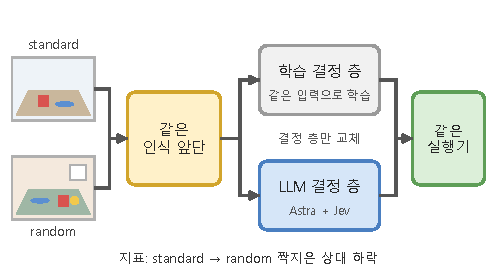
\includegraphics[width=\linewidth]{figures/eval_protocol.pdf}
\caption{\textbf{평가 프로토콜.} 같은 layout의 standard와 random 장면을 짝지어 돌리고 상대 하락(RD)을 잰다. 상위 계획기(Astra, 학습한 8B·35B, 첫 계획 뒤 끔)와 구성(VLA 단독, 상위 단독, 상위 + VLA)을 한 축씩 바꾸고, $\pi_{0.5}$ 미세조정·코드 정책·규칙 기준선을 같은 짝에서 돌린다. 지연 충실 트랙과 동기 공정 트랙을 같은 표에 둔다. 장면 그림은 설명용이다.}
\label{fig:eval}
\end{figure}

주 지표는 같은 layout의 standard와 random을 짝지어 계산한 상대 하락이다.
\begin{equation}
  \mathrm{RD} = 1-\frac{\mathrm{Succ}_{\text{random}}}{\mathrm{Succ}_{\text{standard}}}.
\end{equation}
절대 성공률의 우위는 주장하지 않는다(\cref{fig:eval}). \textbf{H1(시스템)}: PaceNotes의 RD가 $\pi_{0.5}$ 미세조정보다 작다(차의 95\% 상한 $<0$). \textbf{H2(상위 학습)}: 학생 상위 모델의 RD가 Astra 상위와 비열등하다. \textbf{H3(조건부 층)}: VLA 층을 넣었다면, 넣은 판의 RD가 상위 단독보다 크지 않다. 모두 지연 충실 트랙에서 판정한다.

\begin{table*}[t]
\centering
\scriptsize
\setlength{\tabcolsep}{4pt}
\begin{tabular}{@{}lllccccc@{}}
\toprule
범주 & 시스템 & 상위 계획기 & standard 성공(\%) & random 성공(\%) & RD $\downarrow$ & 벽시계(s/판) & 상위 호출/판 \\
\midrule
\multirow{3}{*}{기준선}
 & 코드 정책 (CaP-X식)~\cite{fu2026capx} & Astra & \todoexp & \todoexp & \todoexp & \todoexp & \todoexp \\
 & $\pi_{0.5}$ 미세조정~\cite{pi05_2025} & 없음 & \todoexp & \todoexp & \todoexp & \todoexp & --- \\
 & 규칙 + 스크립트 스킬 & 없음 & \todoexp & \todoexp & \todoexp & \todoexp & --- \\
\midrule
\multirow{4}{*}{PaceNotes 1단계}
 & 상위 + 실행기 & Astra & \todoexp & \todoexp & \todoexp & \todoexp & \todoexp \\
 & \textbf{상위 + 실행기} & 8B 학생 & \todoexp & \todoexp & \todoexp & \todoexp & \todoexp \\
 & \textbf{상위 + 실행기} & 35B 학생, 줄기 D & \todoexp & \todoexp & \todoexp & \todoexp & \todoexp \\
 & \textbf{상위 + 실행기} & 35B 학생, 줄기 R & \todoexp & \todoexp & \todoexp & \todoexp & \todoexp \\
\midrule
PaceNotes 2단계 & 상위 + VLA (트리거 시) & 35B 학생 & \todoexp & \todoexp & \todoexp & \todoexp & \todoexp \\
\bottomrule
\end{tabular}
\caption{\textbf{주 결과 (계획, 지연 충실 트랙; 동기 공정 트랙은 같은 형식으로 병기).} 기대: $\pi_{0.5}$ 미세조정은 standard 성공률이 높지만 RD가 크고, PaceNotes 1단계는 RD가 작다(H1). 학생 상위 모델은 Astra와 비열등하다(H2). 2단계 줄은 트리거가 걸렸을 때만 채운다(H3).}
\label{tab:main}
\end{table*}

\subsection{열린 전제}
\label{sec:premises}
아래 전제가 서기 전까지 설계는 잠정이다(\cref{tab:premises}). 전제가 틀리면 그 칸만 바꾸고 나머지는 유지한다. 1단계 전제(Q1--Q5)를 먼저 검증하고, 2단계 전제(P1--P9)는 층을 다시 넣을 때 검증한다.

\begin{table}[t]
\centering
\scriptsize
\setlength{\tabcolsep}{2pt}
\begin{tabular}{@{}p{0.06\linewidth}p{0.48\linewidth}p{0.42\linewidth}@{}}
\toprule
\# & 아직 확실하지 않은 전제 & 가르는 실험과 지금 상태 \\
\midrule
\multicolumn{3}{@{}l}{\textbf{1단계}} \\
Q1 & 가설 H-L(\cref{sec:hl}) & 초기 근거(8B, DEV \tentative{4/4}); 35B 준비 p50 \tentative{1.11\,s} \\
Q2 & 상위 단독이 분포 밖에서도 버틴다 & E-DIST8, 최종 35B 평가 \\
Q3 & 손으로 준 정보 없이도 된다; 줄기 D·R 중 무엇이 나은가 & E-STRIP8b, E-PT/ND, 최종 35B 두 판 \\
Q4 & 상위 한 호출의 명령이 충분히 정확 & 방향 \tentative{13/13}, 알아채기 \tentative{0/13} \\
Q5 & 지연·비용이 실물 조건에서도 유지 & 실물 단계 \\
\midrule
\multicolumn{3}{@{}l}{\textbf{2단계(조건부)}} \\
P1 & 먼 구간 분기가 실데이터에서도 준수 $\ge0.8$ & 오프라인 \tentative{0.899}(분기 75\%); 폐루프 미측정 \\
P3 & 결합이 트리거한 한계를 줄인다 & 트리거 뒤 V3 \\
P5 & 상위 그리퍼 의도에 VLA가 쥐는 시점을 맞게 정함 & V0 뒤 \\
P7 & 목표$\rightarrow$결정 변환과 연속 혼합이 튀지 않고 도움이 됨 & V2 \\
P9 & 상위 목표가 낡을 때(물체 이동) 혼합이 VLA 쪽으로 옮겨 감 & V2 \\
\bottomrule
\end{tabular}
\caption{\textbf{열린 전제.} 모두 검증 전이며 상태 칸의 값은 초기값이다. 2단계 전제는 정본 §96 보충 5의 결합 방식 기준이며, 나머지(가중 입력의 추정, 정밀도 대가)는 층을 다시 넣을 때 함께 연다.}
\label{tab:premises}
\end{table}
